\section{Hardwarearkitektur (JS)}
Følgende diagrammer beskriver hardwarearkitekturen. 

\subsection{Domænemodel (JS)}
Første del af hardware arkitekturen ligger i at få udarbejdet en domænemodel som er afbildet på figur \ref{lab:Domainmodel}.

\begin{figure}[H]
  \centering
    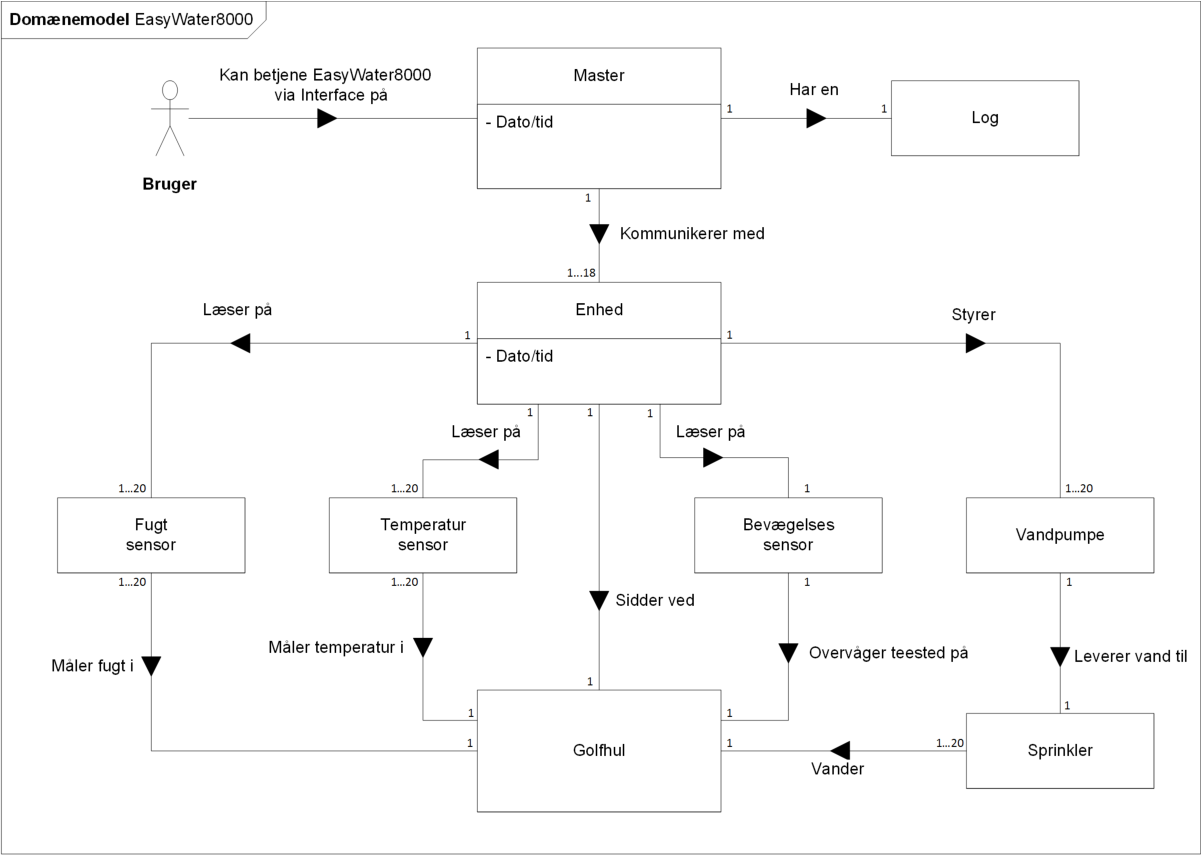
\includegraphics[width=0.75\textwidth]{Billeder/Domainmodel}
    \caption{Domænemodel}
    \label{lab:Domainmodel}
\end{figure}

Dette diagrams formål er at skabe et overbliksbillede for lægmænd, af samme årsag er der ikke anvendt tekniske eller faglige udtryk, men gør brug af tale sprog. Hver kasse repræsenterer en fysisk genstand i systemet og pilene imellem disse beskriver er handling eller sammenhæng imellem disse. 

\subsection{Blokdefinationsdiagram (JS)}
BDD-diagrammer beskriver de overordnet hardware dele i systemet og hvilke dele disse er opbygget af. Et BDD er opbygget i lag, for hver gang en systemdel beskrives som bestående af flere komponenter udvides diagrammet med et lag til beskrivelse af disse dele. Et BDD kan ses på figur \ref{lab:BDD}. 

\begin{figure}[H]
  \centering
    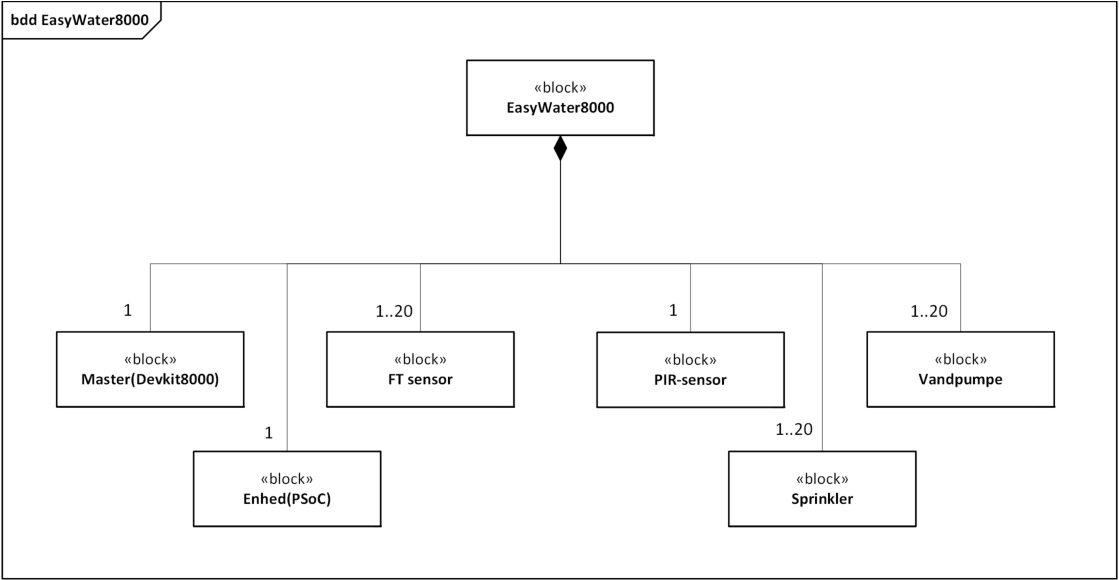
\includegraphics[width=0.75\textwidth]{Billeder/BDD}
    \caption{BDD af EasyWater8000 som samlet system}
    \label{lab:BDD}
\end{figure}

Yderligere ses det at EastWater8000 er opbygget af 6 dele som alle ligger i andet lag og hvor EasyWater8000 alene udgør det øverste lag. Ydermere fortæller tallene ved hver blok hvor mange af disse der fremkommer i systemet. 
Master og Enhed blokkene er så omfattende at disse er beskrevet yderligere med hver deres BDD som kan ses på figur \ref{lab:BDD_Master} og \ref{lab:BDD_Enhed} 

\begin{figure}[H]
\begin{minipage}{0.45\textwidth}
  \centering
    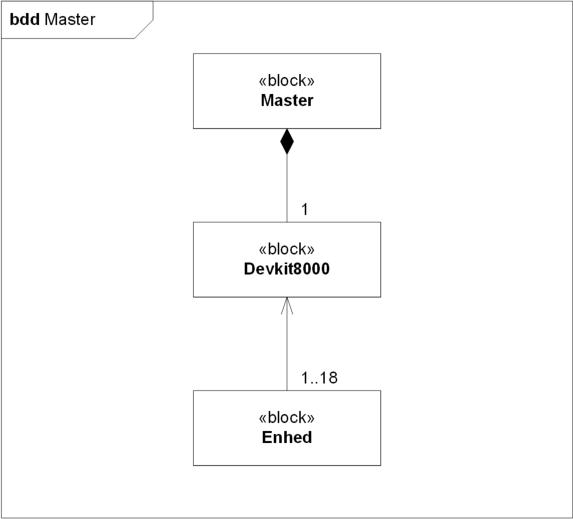
\includegraphics[width=0.75\textwidth]{Billeder/BDD_Master}
    \caption{BDD af Master blokken}
    \label{lab:BDD_Master}
\end{minipage}
\hspace{0.1\textwidth}
\begin{minipage}{0.45\textwidth}
  \centering
    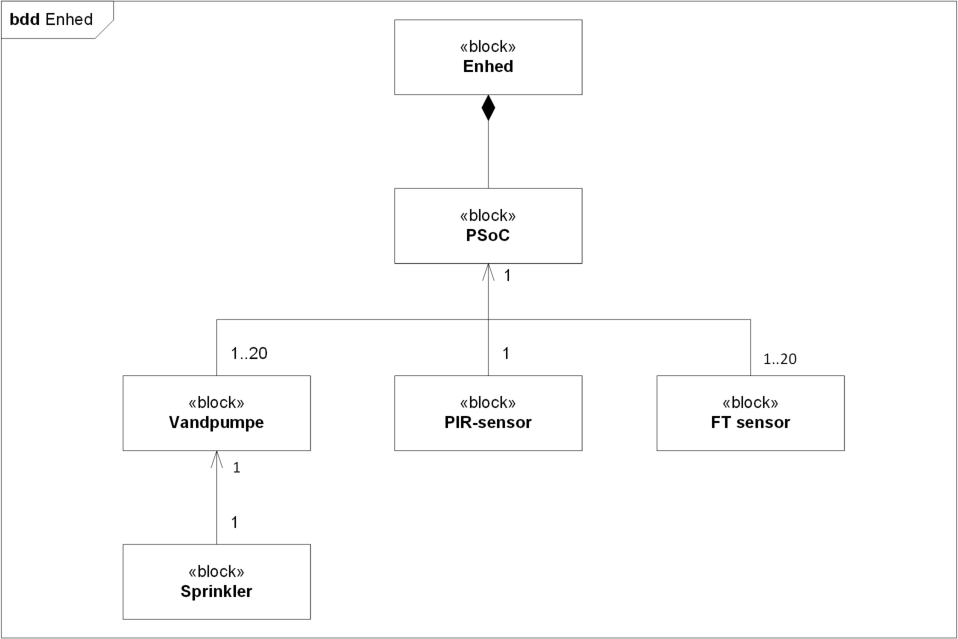
\includegraphics[width=0.75\textwidth]{Billeder/BDD_Enhed}
    \caption{BDD af Enhed blokken}
    \label{lab:BDD_Enhed}
    \end{minipage}
\end{figure}

\subsection{Internt blokdiagram (JS)}
Når blokdiagrammerne er beskrevet færdig er det nødvendigt at definere hvordan disse er forbundet og hvilke signaler der gøres brug af. Dette er beskrevet i et IBD-diagram og et eksempel herfor kan ses på figur \ref{lab:IBD}

\begin{figure}[H]
  \centering
    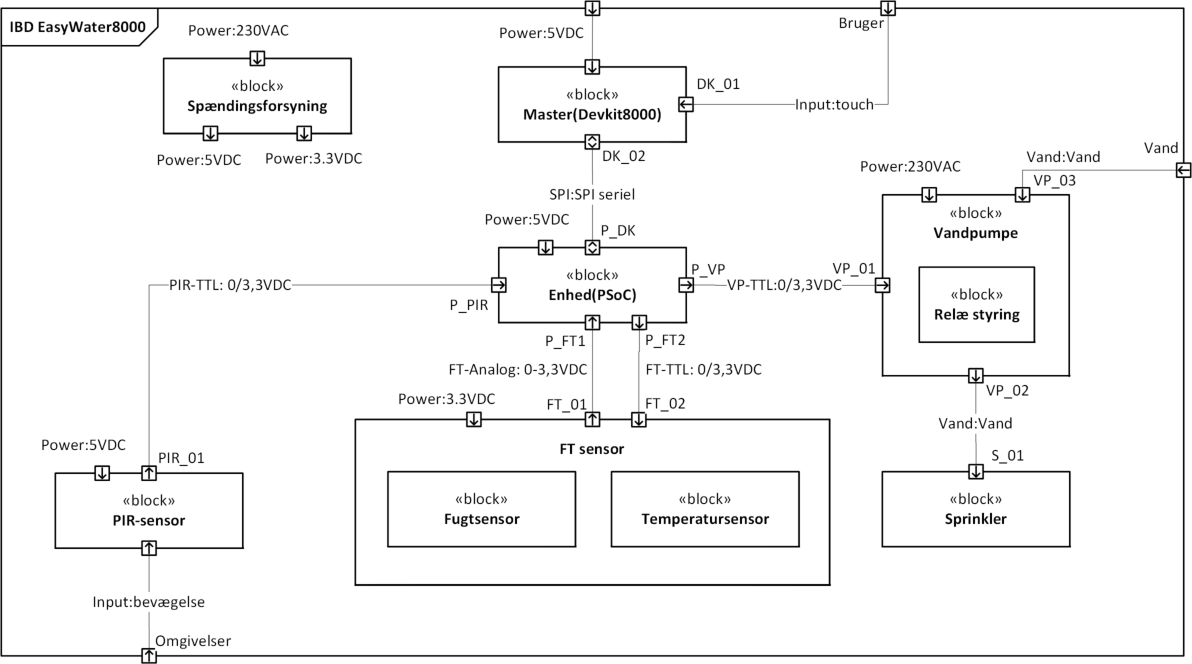
\includegraphics[width=0.75\textwidth]{Billeder/IBD}
    \caption{IBD af EasyWater8000}
    \label{lab:IBD}
\end{figure}

I dette diagram bliver alle signaler og porte tildelt navne og typer, det er ud fra disse at designet bliver lavet. Ikke alle porte er tilsluttet et elektrisk signal, disse kan også styre andre elementer som skal transporteres rundt i systemet. EasyWater8000 gør f.eks. brug af en port til styring af vand.